\documentclass[]{BasiliskReportMemo}
\usepackage{AVS}

\newcommand{\submiterInstitute}{Autonomous Vehicle Simulation (AVS) Laboratory,\\ University of Colorado}

\newcommand{\ModuleName}{extForceTorque}
\newcommand{\subject}{Module to apply a prescribed Force or Torque onto a Rigid Body}
\newcommand{\status}{First Version}
\newcommand{\preparer}{H. Schaub}
\newcommand{\summary}{This module allows an external force and/or torque about a body fixed point $B$ to be prescribed through either direct input from python, or through a message.     }


\begin{document}


\makeCover


%
%	enter the revision documentation here
%	to add more lines, copy the table entry and the \hline, and paste after the current entry.
%
\pagestyle{empty}
{\renewcommand{\arraystretch}{1.1}
\noindent
\begin{longtable}{|p{0.5in}|p{4.5in}|p{1.14in}|}
\hline
{\bfseries Rev}: & {\bfseries Change Description} & {\bfseries By} \\
\hline
v1.0 & Initial document & H. Schaub \\
\hline

\end{longtable}
}

\newpage
\setcounter{page}{1}
\pagestyle{fancy}

\tableofcontents
~\\ \hrule ~\\


\begin{figure}[htb]
	\centerline{
	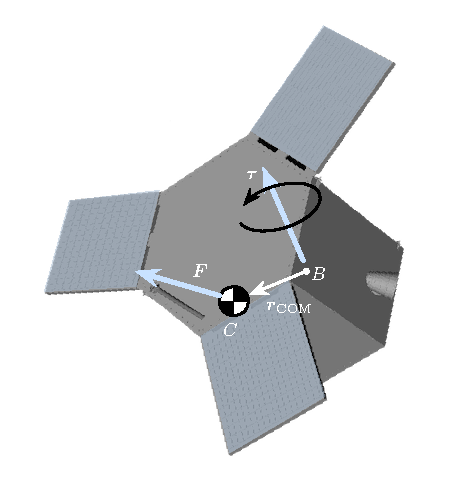
\includegraphics[]{Figures/ForceTorqueDiagram}
	}
	\caption{Illustration of Force and Torque acting on a rigid body}
	\label{fig:forceTorque}
\end{figure}
\section{Introduction}
This module allows a general force $\bm F$ or torque $\bm \tau$ to be applied onto a rigid body.  The force is the net external force acting through the center of mass, and can be specified in inertial $\mathcal{N}$ or body-frame $\mathcal{B}$ coordinates.  The torque is taken about the body-fixed point $B$, and the vector components are given in the body frame $\mathcal{B}$.


\section{Specifying the Forces/Torques through Messages}
The module reads in a message that specifies  an external force or external torque.  Not that there essentially are  3 input options.  The torque vector is always provided in body frame vector components.  The external force can be provided as a vector with respect to the inertial or body frame.  {\bfseries Note, it is possible to set both types, but this applies 2 separate vectors to the rigid body.}

\subsection{External Torque}
The torque message $\leftexp{B}{\bm\tau}_{B}$ is stored in a message with default name 

{\tt extTorquePntB\_B\_cmds}

\noindent stored in the module variable 

{\tt cmdTorqueInMsgName}

\subsection{External Force in $\mathcal{N}$ Inertial Frame Vector Components}
The inertial force message $\leftexp{N}{\bm F}$ is stored in a message with default name 

{\tt extForce\_N\_cmds}

\noindent stored in the module variable 

{\tt cmdForceInertialInMsgName}


\subsection{External Force in $\mathcal{B}$ Body Frame Vector Components}
The inertial force message $\leftexp{B}{\bm F}$ is stored in a message with default name 

{\tt extForce\_B\_cmds}

\noindent stored in the module variable 

{\tt cmdForceBodyInMsgName}






\section{Module Parameters}
The forces and torque vectors  can also be set directly from python.  These values are added up in addition ot the messages set above.


\subsection{{\tt extTorquePntB\_B} Parameter}
This vector sets the external torque, about point $B$, in $\mathcal{B}$ body-frame vector components.

\subsection{{\tt extForce\_N} Parameter}
This vector sets the external force $\bm F$ in $\mathcal{N}$ inertial-frame vector components.

\subsection{{\tt extForce\_B} Parameter}
This vector sets the external force $\bm F$ in $\mathcal{B}$ inertial-frame vector components.





\end{document}
